% GENERATED by benchmarks/scripts/crossarch.py -- do not edit.
% artifact:   fig_crossarch_stages (figure)
% set:        x86_64/current on a2 @ 18d0f83627b5 (2026-09-12)
% set:        aarch64/current on galaxy @ 18d0f83627b5 (2026-09-12)
% reference:  x86_64 (every delta is against this)
% inputs:     sha256:32da7e14ac55e610
% provenance: paper/generated/cross-arch/PROVENANCE.md#fig_crossarch_stages
%
\begin{figure}[tb]
\centering
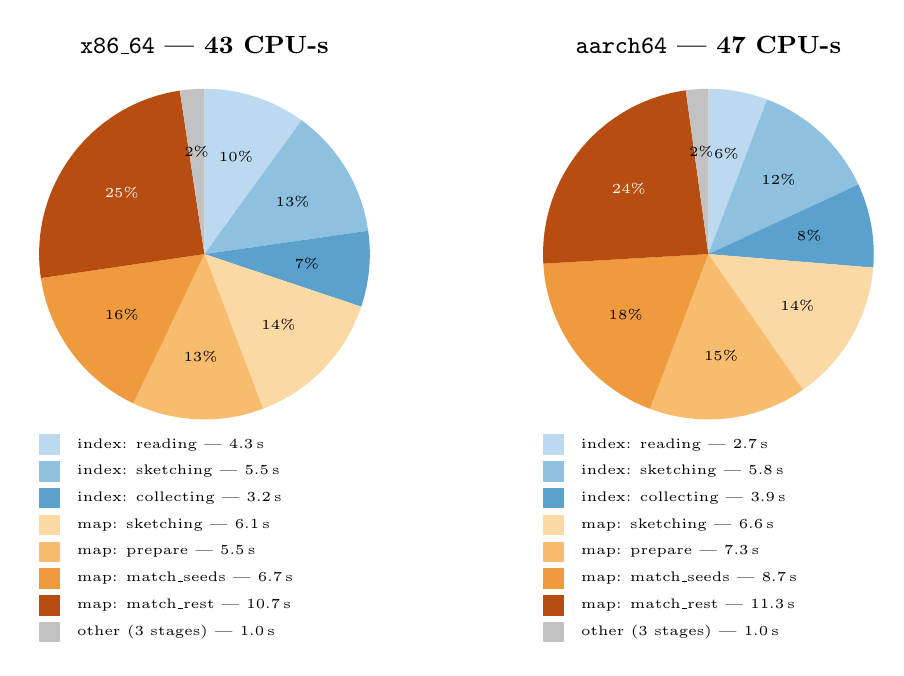
\begin{tikzpicture}[x=1cm,y=1cm]
\node[font=\small\bfseries] at (0.00,2.65) {\texttt{x86\_64} — 43 CPU-s};
\definecolor{p0c0}{HTML}{BCD9EF}
\definecolor{p0c1}{HTML}{8EC0E0}
\definecolor{p0c2}{HTML}{5AA2CD}
\definecolor{p0c3}{HTML}{FBD9A5}
\definecolor{p0c4}{HTML}{F7BC6D}
\definecolor{p0c5}{HTML}{F09A3E}
\definecolor{p0c6}{HTML}{B74D10}
\definecolor{p0c7}{HTML}{C2C2C2}
\fill[p0c0] (0.00,0.00) -- ++(90.000:2.10) arc[start angle=90.000, end angle=54.054, radius=2.10] -- cycle;
\node[font=\tiny,text=black] at (0.40,1.24) {10\%};
\fill[p0c1] (0.00,0.00) -- ++(54.054:2.10) arc[start angle=54.054, end angle=8.108, radius=2.10] -- cycle;
\node[font=\tiny,text=black] at (1.12,0.67) {13\%};
\fill[p0c2] (0.00,0.00) -- ++(8.108:2.10) arc[start angle=8.108, end angle=-18.540, radius=2.10] -- cycle;
\node[font=\tiny,text=black] at (1.30,-0.12) {7\%};
\fill[p0c3] (0.00,0.00) -- ++(-18.540:2.10) arc[start angle=-18.540, end angle=-69.232, radius=2.10] -- cycle;
\node[font=\tiny,text=black] at (0.94,-0.90) {14\%};
\fill[p0c4] (0.00,0.00) -- ++(-69.232:2.10) arc[start angle=-69.232, end angle=-115.472, radius=2.10] -- cycle;
\node[font=\tiny,text=black] at (-0.05,-1.30) {13\%};
\fill[p0c5] (0.00,0.00) -- ++(-115.472:2.10) arc[start angle=-115.472, end angle=-171.662, radius=2.10] -- cycle;
\node[font=\tiny,text=black] at (-1.05,-0.77) {16\%};
\fill[p0c6] (0.00,0.00) -- ++(-171.662:2.10) arc[start angle=-171.662, end angle=-261.422, radius=2.10] -- cycle;
\node[font=\tiny,text=white] at (-1.05,0.78) {25\%};
\fill[p0c7] (0.00,0.00) -- ++(-261.422:2.10) arc[start angle=-261.422, end angle=-270.000, radius=2.10] -- cycle;
\node[font=\tiny,text=black] at (-0.10,1.30) {2\%};
\fill[p0c0] (-2.10,-2.55) rectangle ++(0.26,0.26);
\node[anchor=west,font=\tiny] at (-1.74,-2.42) {index: reading — 4.3\,s};
\fill[p0c1] (-2.10,-2.89) rectangle ++(0.26,0.26);
\node[anchor=west,font=\tiny] at (-1.74,-2.76) {index: sketching — 5.5\,s};
\fill[p0c2] (-2.10,-3.23) rectangle ++(0.26,0.26);
\node[anchor=west,font=\tiny] at (-1.74,-3.10) {index: collecting — 3.2\,s};
\fill[p0c3] (-2.10,-3.57) rectangle ++(0.26,0.26);
\node[anchor=west,font=\tiny] at (-1.74,-3.44) {map: sketching — 6.1\,s};
\fill[p0c4] (-2.10,-3.91) rectangle ++(0.26,0.26);
\node[anchor=west,font=\tiny] at (-1.74,-3.78) {map: prepare — 5.5\,s};
\fill[p0c5] (-2.10,-4.25) rectangle ++(0.26,0.26);
\node[anchor=west,font=\tiny] at (-1.74,-4.12) {map: match\_seeds — 6.7\,s};
\fill[p0c6] (-2.10,-4.59) rectangle ++(0.26,0.26);
\node[anchor=west,font=\tiny] at (-1.74,-4.46) {map: match\_rest — 10.7\,s};
\fill[p0c7] (-2.10,-4.93) rectangle ++(0.26,0.26);
\node[anchor=west,font=\tiny] at (-1.74,-4.80) {other (3 stages) — 1.0\,s};
\node[font=\small\bfseries] at (6.40,2.65) {\texttt{aarch64} — 47 CPU-s};
\definecolor{p1c0}{HTML}{BCD9EF}
\definecolor{p1c1}{HTML}{8EC0E0}
\definecolor{p1c2}{HTML}{5AA2CD}
\definecolor{p1c3}{HTML}{FBD9A5}
\definecolor{p1c4}{HTML}{F7BC6D}
\definecolor{p1c5}{HTML}{F09A3E}
\definecolor{p1c6}{HTML}{B74D10}
\definecolor{p1c7}{HTML}{C2C2C2}
\fill[p1c0] (6.40,0.00) -- ++(90.000:2.10) arc[start angle=90.000, end angle=69.237, radius=2.10] -- cycle;
\node[font=\tiny,text=black] at (6.63,1.28) {6\%};
\fill[p1c1] (6.40,0.00) -- ++(69.237:2.10) arc[start angle=69.237, end angle=24.910, radius=2.10] -- cycle;
\node[font=\tiny,text=black] at (7.29,0.95) {12\%};
\fill[p1c2] (6.40,0.00) -- ++(24.910:2.10) arc[start angle=24.910, end angle=-4.690, radius=2.10] -- cycle;
\node[font=\tiny,text=black] at (7.68,0.23) {8\%};
\fill[p1c3] (6.40,0.00) -- ++(-4.690:2.10) arc[start angle=-4.690, end angle=-55.121, radius=2.10] -- cycle;
\node[font=\tiny,text=black] at (7.53,-0.65) {14\%};
\fill[p1c4] (6.40,0.00) -- ++(-55.121:2.10) arc[start angle=-55.121, end angle=-110.721, radius=2.10] -- cycle;
\node[font=\tiny,text=black] at (6.56,-1.29) {15\%};
\fill[p1c5] (6.40,0.00) -- ++(-110.721:2.10) arc[start angle=-110.721, end angle=-176.684, radius=2.10] -- cycle;
\node[font=\tiny,text=black] at (5.35,-0.77) {18\%};
\fill[p1c6] (6.40,0.00) -- ++(-176.684:2.10) arc[start angle=-176.684, end angle=-262.128, radius=2.10] -- cycle;
\node[font=\tiny,text=white] at (5.39,0.83) {24\%};
\fill[p1c7] (6.40,0.00) -- ++(-262.128:2.10) arc[start angle=-262.128, end angle=-270.000, radius=2.10] -- cycle;
\node[font=\tiny,text=black] at (6.31,1.30) {2\%};
\fill[p1c0] (4.30,-2.55) rectangle ++(0.26,0.26);
\node[anchor=west,font=\tiny] at (4.66,-2.42) {index: reading — 2.7\,s};
\fill[p1c1] (4.30,-2.89) rectangle ++(0.26,0.26);
\node[anchor=west,font=\tiny] at (4.66,-2.76) {index: sketching — 5.8\,s};
\fill[p1c2] (4.30,-3.23) rectangle ++(0.26,0.26);
\node[anchor=west,font=\tiny] at (4.66,-3.10) {index: collecting — 3.9\,s};
\fill[p1c3] (4.30,-3.57) rectangle ++(0.26,0.26);
\node[anchor=west,font=\tiny] at (4.66,-3.44) {map: sketching — 6.6\,s};
\fill[p1c4] (4.30,-3.91) rectangle ++(0.26,0.26);
\node[anchor=west,font=\tiny] at (4.66,-3.78) {map: prepare — 7.3\,s};
\fill[p1c5] (4.30,-4.25) rectangle ++(0.26,0.26);
\node[anchor=west,font=\tiny] at (4.66,-4.12) {map: match\_seeds — 8.7\,s};
\fill[p1c6] (4.30,-4.59) rectangle ++(0.26,0.26);
\node[anchor=west,font=\tiny] at (4.66,-4.46) {map: match\_rest — 11.3\,s};
\fill[p1c7] (4.30,-4.93) rectangle ++(0.26,0.26);
\node[anchor=west,font=\tiny] at (4.66,-4.80) {other (3 stages) — 1.0\,s};
\end{tikzpicture}
\caption{Where the CPU time goes on each machine, benchmark B01 (Containment, -@1). Indexing is blue, mapping orange, and wedges under 5\% are folded into a single grey 'other'. Read against Table~\ref{tab:xarch:stages}, which carries every benchmark.}
\label{fig:xarch:stages}
\end{figure}
